\section{Intrinsische Halbwertsbreite des HPGe-Halbleiterdetektors}
\begin{figure}[htbp]
    \centering

    \begin{subfigure}[t]{0.48\textwidth}
        \centering
        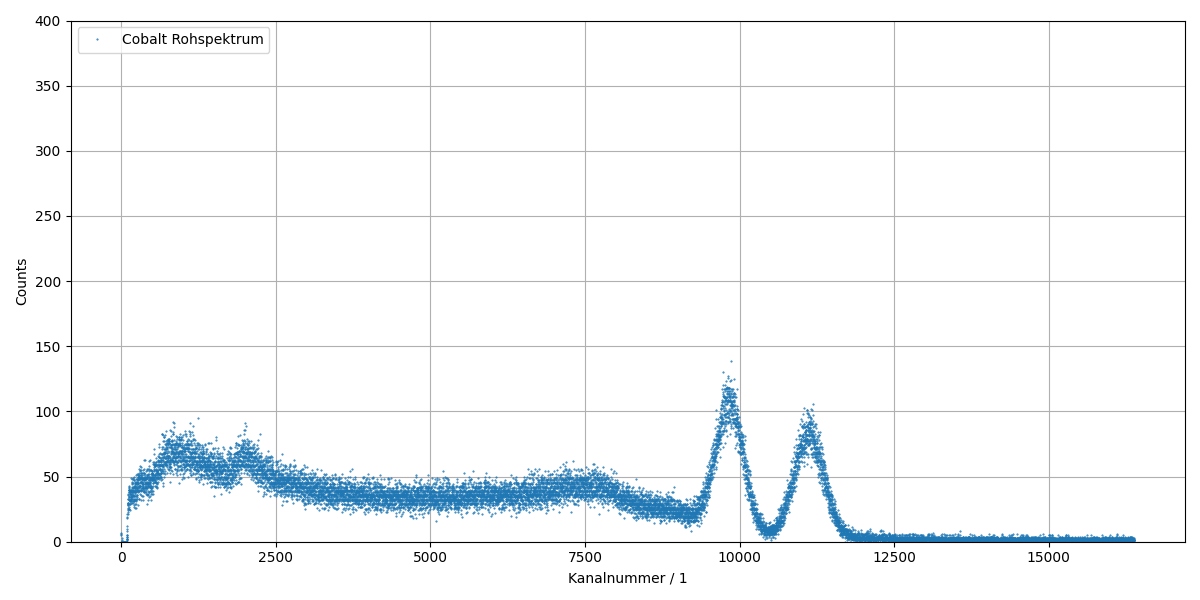
\includegraphics[width=\linewidth]{figs/Cobalt_roh.png}
        \caption{NaI-Szintillationsdetektor}
        \label{fig:}
    \end{subfigure}
    \hfill
    \begin{subfigure}[t]{0.48\textwidth}
        \centering
        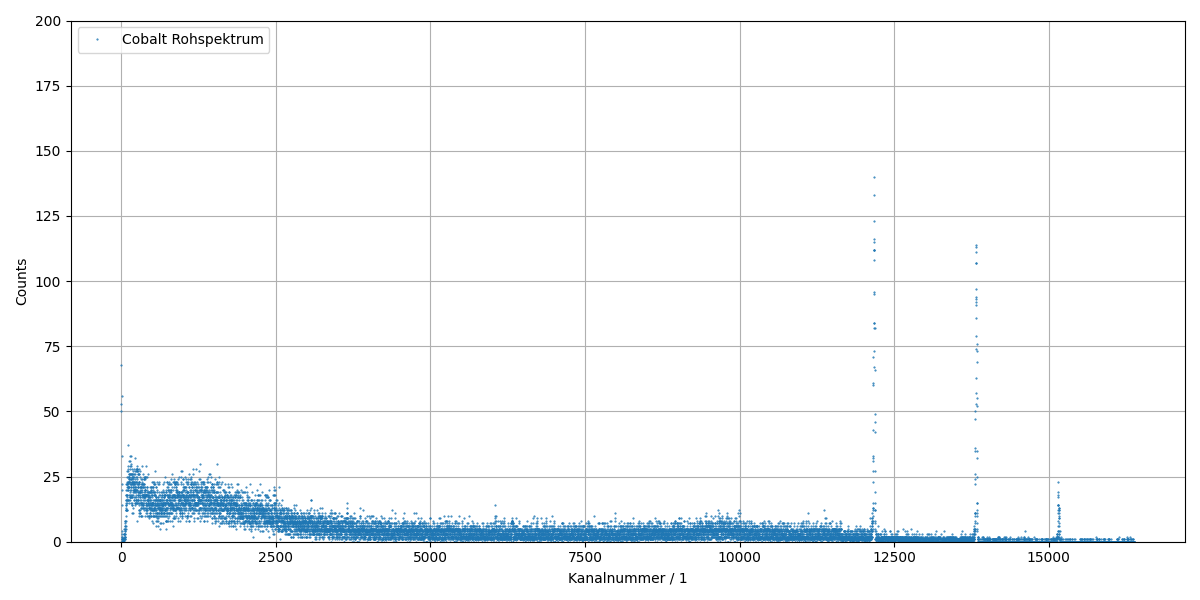
\includegraphics[width=\linewidth]{figs/Ge_Cobalt_roh.png}
        \caption{HPGe-Halbleiterdetektor}
        \label{fig:}
    \end{subfigure}
    
    \caption{}
    \label{fig:anhang_1}
\end{figure}
\begin{figure}[htbp]
    \centering

    \begin{subfigure}[t]{0.48\textwidth}
        \centering
        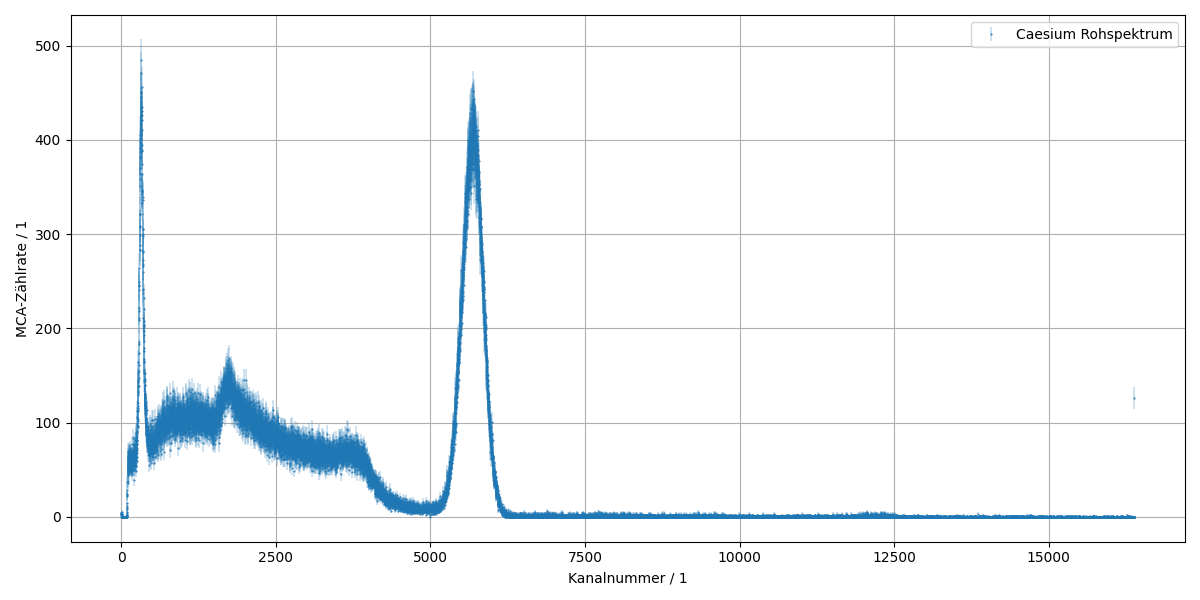
\includegraphics[width=\linewidth]{figs/Caesium_roh.png}
        \caption{NaI-Szintillationsdetektor}
        \label{fig:}
    \end{subfigure}
    \hfill
    \begin{subfigure}[t]{0.48\textwidth}
        \centering
        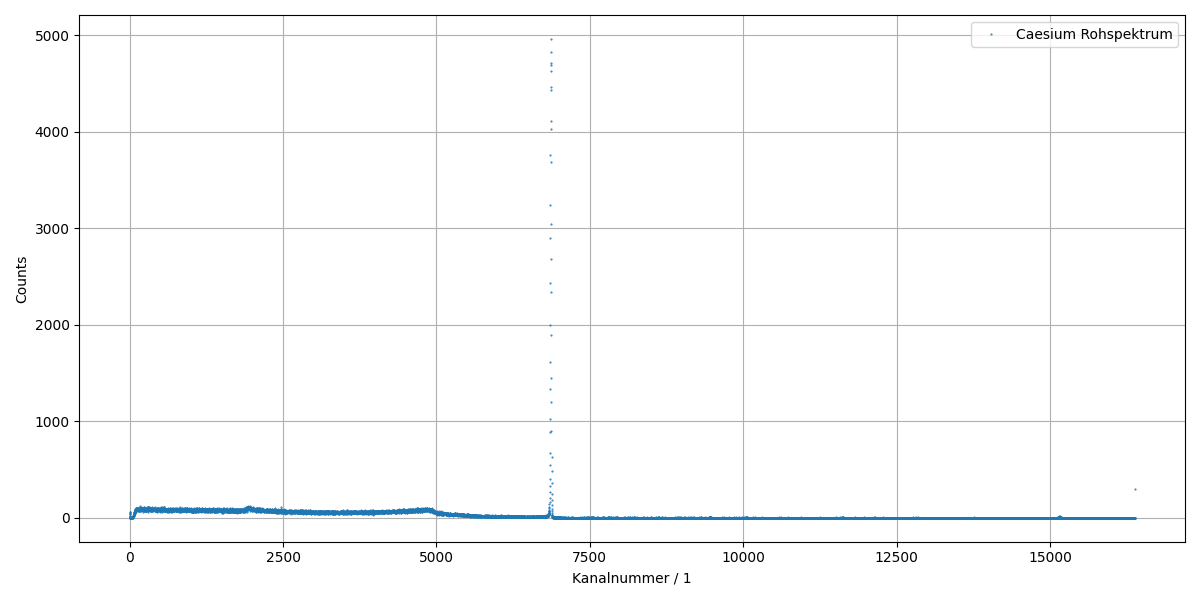
\includegraphics[width=\linewidth]{figs/Ge_Caesium_roh.png}
        \caption{HPGe-Halbleiterdetektor}
        \label{fig:}
    \end{subfigure}
    
    \caption{}
    \label{fig:anhang_1}
\end{figure}
\begin{figure}[htbp]
    \centering

    \begin{subfigure}[t]{0.48\textwidth}
        \centering
        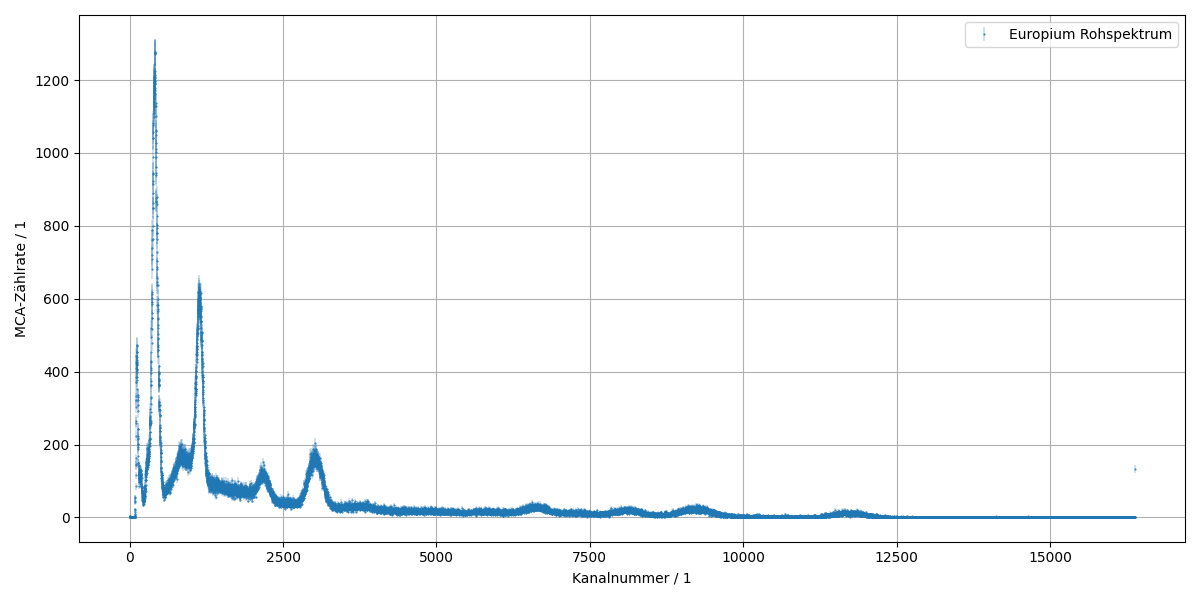
\includegraphics[width=\linewidth]{figs/Europium_roh.png}
        \caption{NaI-Szintillationsdetektor}
        \label{fig:}
    \end{subfigure}
    \hfill
    \begin{subfigure}[t]{0.48\textwidth}
        \centering
        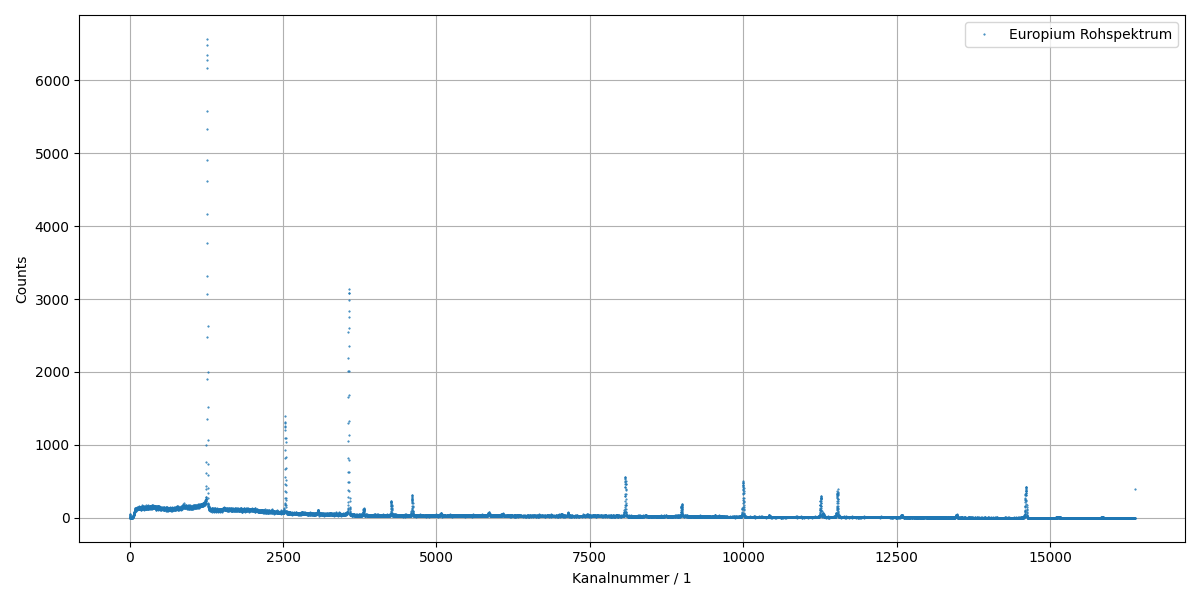
\includegraphics[width=\linewidth]{figs/Ge_europium_roh.png}
        \caption{HPGe-Halbleiterdetektor}
        \label{fig:}
    \end{subfigure}
    
    \caption{}
    \label{fig:anhang_1}
\end{figure}